% 2016 全国卷Ⅰ理科第 6 题：三个圆形投影及各自的两条垂直半径。
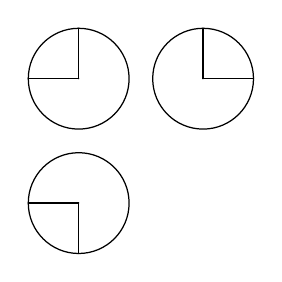
\begin{tikzpicture}[line width=.45pt,line cap=round,line join=round]
  \coordinate (upperleft) at (0,0);
  \coordinate (upperright) at (1.58,0);
  \coordinate (lowerleft) at (0,-1.58);
  \def\r{.64}
  \draw (upperleft) circle[radius=\r];
  \draw (upperright) circle[radius=\r];
  \draw (lowerleft) circle[radius=\r];
  \draw (upperleft) -- (0,\r) (-\r,0) -- (upperleft);
  \draw (upperright) -- (1.58,\r) (upperright) -- (1.58+\r,0);
  \draw (lowerleft) -- (-\r,-1.58) (lowerleft) -- (0,-1.58-\r);
\end{tikzpicture}
